\section{Introduction}\label{sec:introduction}

In 2009, Bitcoin \cite{bitcoin2009} introduced a new notion of decentralized cryptocurrency and trustless transaction processing. This is facilitated by blockchain, which introduced a new way for mistrusting agents to cooperate without trusted third parties. This was followed by Ethereum \cite{ethereum2014}, which introduced generalized scripting functionality, allowing `smart contracts' that execute algorithmically in a verifiable and somewhat trustless manner. Cryptocurrencies promise notions of cryptographic security, privacy, incentive alignment, digital usability, and open accessibility while removing most facets of counterparty risk. However, as these cryptocurrencies are, by their nature, unbacked by governments or physical assets, and the technology is quite new and developing, their prices are subject to wild volatility, which affects their usability.


A stablecoin is a cryptocurrency with an economic structure built on top of blockchain that aims to stabilize the purchasing power of the coin. A true stablecoin, often referred to as the ``Holy Grail of crypto'', would offer the benefits of cryptocurrencies without the unusable volatility and remains elusive. A more tangible goal is to design a stablecoin that maximizes the probability of remaining stable long-term. If one can establish guarantees for the stability of such a stablecoin, this would be a significant step toward forming a robust decentralized financial system and facilitating economic adoption of cryptocurrencies.



\paragraph{Cryptocurrency volatility.}
Cryptocurrencies face difficult technological, usability, and regulatory challenges to be successful long-term. Many cryptocurrency systems develop different approaches to solving these problems. Even assuming the space is long-term successful, there is large uncertainty about the long-term value of individual systems.

The value of these systems depends on network effects: value changes in a nonlinear way as new participants join. In concrete terms, the more people who use the system, the more likely it can be used to fulfill a given real world transaction. The success of a cryptocurrency relies on a mass of agents--e.g., consumers, businesses, and/or financial institutions--adopting the system for economic transactions and value storage. Which systems will achieve this adoption is highly uncertainty, and so current cryptocurrency positions are very speculative bets on new technology. Further, cryptocurrency markets face limited liquidity and market manipulation. In addition, the decentralized control and privacy features of cryptocurrencies can be at odds with desires of governments, which introduces further uncertainty around attempted interventions in the space.

These uncertainties drive price volatility, which feeds back into fundamental usability problems. It makes cryptocurrencies unusable as short-term stores of value and means of payment, which increases the barriers to adoption. Indeed, today we see that most cryptocurrency transactions represent speculative investment as opposed to typical economic activity.


\paragraph{Stablecoins.}
Stablecoins aim to bootstrap price stability into cryptocurrencies as a stop-gap measure for adoption. Current projects take one of two forms:
\begin{itemize}
	\item \textbf{Custodial stablecoins} rely on trusted institutions to hold reserve assets off-chain (e.g., \$1 per coin). This introduces counterparty risk that cryptocurrencies otherwise solve.
	\item \textbf{Non-custodial (or decentralized) stablecoins} create on-chain risk transfer markets via complex systems of algorithmic financial contracts backed by volatile cryptoassets.
\end{itemize}
We focus on non-custodial stablecoins and, more generally, the stable asset and risk transfer markets that they represent. Non-custodial systems are not well understood whereas custodial stablecoins can be interpreted using existing well-developed financial literature. Further, non-custodial stablecoins operate in the public/permissionless blockchain setting, in which any agent can participate. In this setting, malicious agents can participate in stablecoin systems. As we will see, this can introduce new economic attacks.



\subsection{Non-custodial (decentralized) stablecoins}

The non-custodial stablecoins that we consider create systems of contracts on-chain with the following features encoded in the protocol. We refer to these as \textbf{DStablecoins}.
\begin{itemize}
	\item Risk is transferred from stablecoin holders to speculators. Stablecoin holders receive a form of price insurance whereas speculators expect a risky return from a leveraged position.\footnote{`Leverage' means that the speculator holds $>1\times$ their initial assets but faces new liabilities.}
	\item Collateral is held in the form of cryptoassets, which backs the stable and risky positions.
	\item An oracle provides pricing information from off-chain markets.
	\item A dynamic deleveraging process balances positions if collateral value deviates too much.
	\item Agents can change their positions through some pre-defined process.
\end{itemize}
These systems are non-custodial (or decentralized) because the contract execution and collateral are all completely on-chain; thus they potentially inherit all of the benefits of cryptocurrencies, such as minimization of counterparty risk. DStablecoins are variants on contracts for difference, which we describe next. The risk transfer typically works by setting up a tranche structure in which losses (or gains) are borne by the speculators and the stablecoin holder holds an instrument like senior debt.\footnote{Intuitively, these are like collateralized debt obligations (CDOs) with the important addition of dynamic deleveraging according to the rules of the protocol. As we will see, it is critical to understand deleveraging spirals as they affect the senior tranches.} There are also other \emph{non-collateralized} (or \emph{algorithmic}) stablecoins--for a discussion of these, see \cite{blockchain2019}. We don't consider these directly in this paper; however, we discuss in Section~\ref{sec:discussion} how our model can accommodate these systems as well.



\paragraph{Contract for difference.} Two parties enter an overcollateralized contract, in which the speculator pays the buyer the difference (possibly negative) between the current value of a risky asset and its value at contract termination.\footnote{Intuitively, this is similar to a forward contract except that the price is only fixed in fiat terms while payout is in the units of the underlying collateral.} For example, a buyer might enter 1 Ether into the contract and a speculator might enter 1 Ether as collateral. At termination, the contract Ether is used to pay the buyer the original dollar value of the 1 Ether at the time of entry. Any excess goes to the speculator. If the contract approaches undercollateralization (if Ether price plummets), the buyer can trigger early settlement or the speculator can add more collateral.


\paragraph{Variants on contracts for difference.}
DStablecoins differ from basic contracts for difference in that (1) the contracts are multi-period and agents can change their positions over time, (2) the positions are dynamically deleveraged according to the protocol, and (3) settlement times are random and dependent on the protocol and agent decisions. The typical mechanics of these contracts are as follows:
\begin{itemize}
	\item Speculators lock cryptoassets in a smart contract, after which they can create new stablecoins as liabilities against their collateral up to a threshold. These stablecoins are sold to stablecoin holders for additional cryptoassets, thus leveraging their positions.
	
	\item At any time, if the collateralization threshold is surpassed, the system attempts to liquidate the speculator's collateral to repurchase stablecoins/reduce leverage.
	
	\item The stablecoin price target is provided by an oracle. The target is maintained by a dynamic coin supply based on an `arbitrage' idea. Notably, this is not true arbitrage as it is based on assumptions about the future value of the collateral.
	\begin{itemize}
		\item If price is above target, speculators have increased incentive to create new coins and sell them at the `premium price'.
		
		\item If price is below target, speculators have increased incentive to repurchase coins (reducing supply) to decrease leverage `at a discount'.
	\end{itemize}
	
	\item Stablecoins are redeemable for collateral through some process. This can take the form of global settlement, in which stakeholders can vote to liquidate the entire system, or direct redemption for individual coins. Settlement can take 24 hours-1 week.
	
	\item Additionally, the system may be able to sell new ownership/decision-making shares as a last attempt to recapitalize a failing system -- e.g., the role of MKR in \href{https://makerdao.com/dai}{Dai} (see \cite{dai_white2017}).
\end{itemize}


\paragraph{DStablecoin risks.}
DStablecoins face two substantial risks:
\begin{enumerate}
	\item Risk of market collapse,
	\item Oracle/governance manipulation.
\end{enumerate}
Our model in this paper focuses on market collapse risk. We further remark on oracle/governance manipulation in Section~\ref{sec:discussion}.

\paragraph{Existing DStablecoins.}
At the time of initial writing in 2019, major non-custodial stablecoins included Dai, BitShares Market Pegged Assets (like bitUSD), and Steem Dollars. In the latter, Steem market cap is essentially collateral; Steem Dollars can be redeemed for \$1 worth of newly minted Steem, and so redemptions affect all Steem hodlers via inflation. Since then, many new stablecoins have arisen based on similar ideas by UMA, Reflexer, and Liquity, as well as \emph{endogenous collateral} stablecoins like Synthetix sUSD, Terra UST, and Celo Dollar (see \cite{klagesmundt2020stablecoins} for further discussion). Notably, unlike custodial stablecoins, Dai is not currently considered as emoney or payment method subject to the Payment Services Directive in the European Union since there is no single issuer or custodian. Thus it does not have AML/KYC requirements.

In an academic white paper, \cite{cao2018} proposed a variation on cryptocurrency-collateralized DStablecoin design. It standardizes the speculative positions by restricting leverage to pre-defined bounds using automated resets. A consequence of these leverage resets is that stablecoin holders are partially liquidated from their positions during downward resets--i.e., when leverage rises above the allowed band due to  a cryptocurrency price crash. This compares with Dai, in which stablecoin holders are only liquidated in global settlement. An effect of this difference is that, in order to maintain a stablecoin position in the short-term, stablecoin holders need to re-buy into stablecoins (at a possibly inflated price) after downward resets. Of the many designs, it is unclear which deleveraging method would lead to a system that survives longer. This motivates us to study the dynamics of DStablecoin systems.


Non-custodial stablecoins have now experienced a wide array of volatility events, failures, and attacks.
Since the initial release of this paper in 2019, Black Thursday in March 2020 saw massive liquidation events result in a substantial depegging in Dai \cite{maker_spiral2020}, mirroring our results in Sections~\ref{sec:dynamics}-\ref{sec:stable_v_unstable}, and miner mempool manipulation that contributed to Dai liquidation auctions clearing at near zero prices at a cost of \$8m to the Maker system \cite{blocknative2020}, mirroring attack surfaces we described in Section~\ref{sec:attacks}.
Prior to this, as discussed in \cite{klagesmundt2018state}, \href{https://nubits.com/}{Nubits} has traded at cents on the dollar since 2018 (Figure~\ref{fig:nubits_chart}), and bitUSD and Steem Dollars have broken their USD pegs periodically (Figure~\ref{fig:bitusd_chart}).
Many additional examples of stablecoin mechanism failures and exploitations occurred through the rest of 2020 (see \cite{klagesmundt2020stablecoins,werner2021sok}).
%Despite these problems, there is a large interest to develop new non-custodial stablecoins. For instance, \href{https://www.basis.io/}{Basis} raised \$133m in 2018 (although it has since closed down), two other projects raised \$32m each, and many other projects raised several million \cite{blockchain2019}.
Yet, the stablecoin space has remained heated with projects such as Dai growing rapidly and many new contenders arising, including UMA, Reflexer, Celo, and Liquity. The work in this paper has proven consequential for the progression of these projects (e.g., \cite{theblock_Maker2019,awesomeMakerDAO}).




\begin{figure}
	\centering
	\begin{subfigure}[b]{0.4\textwidth}
		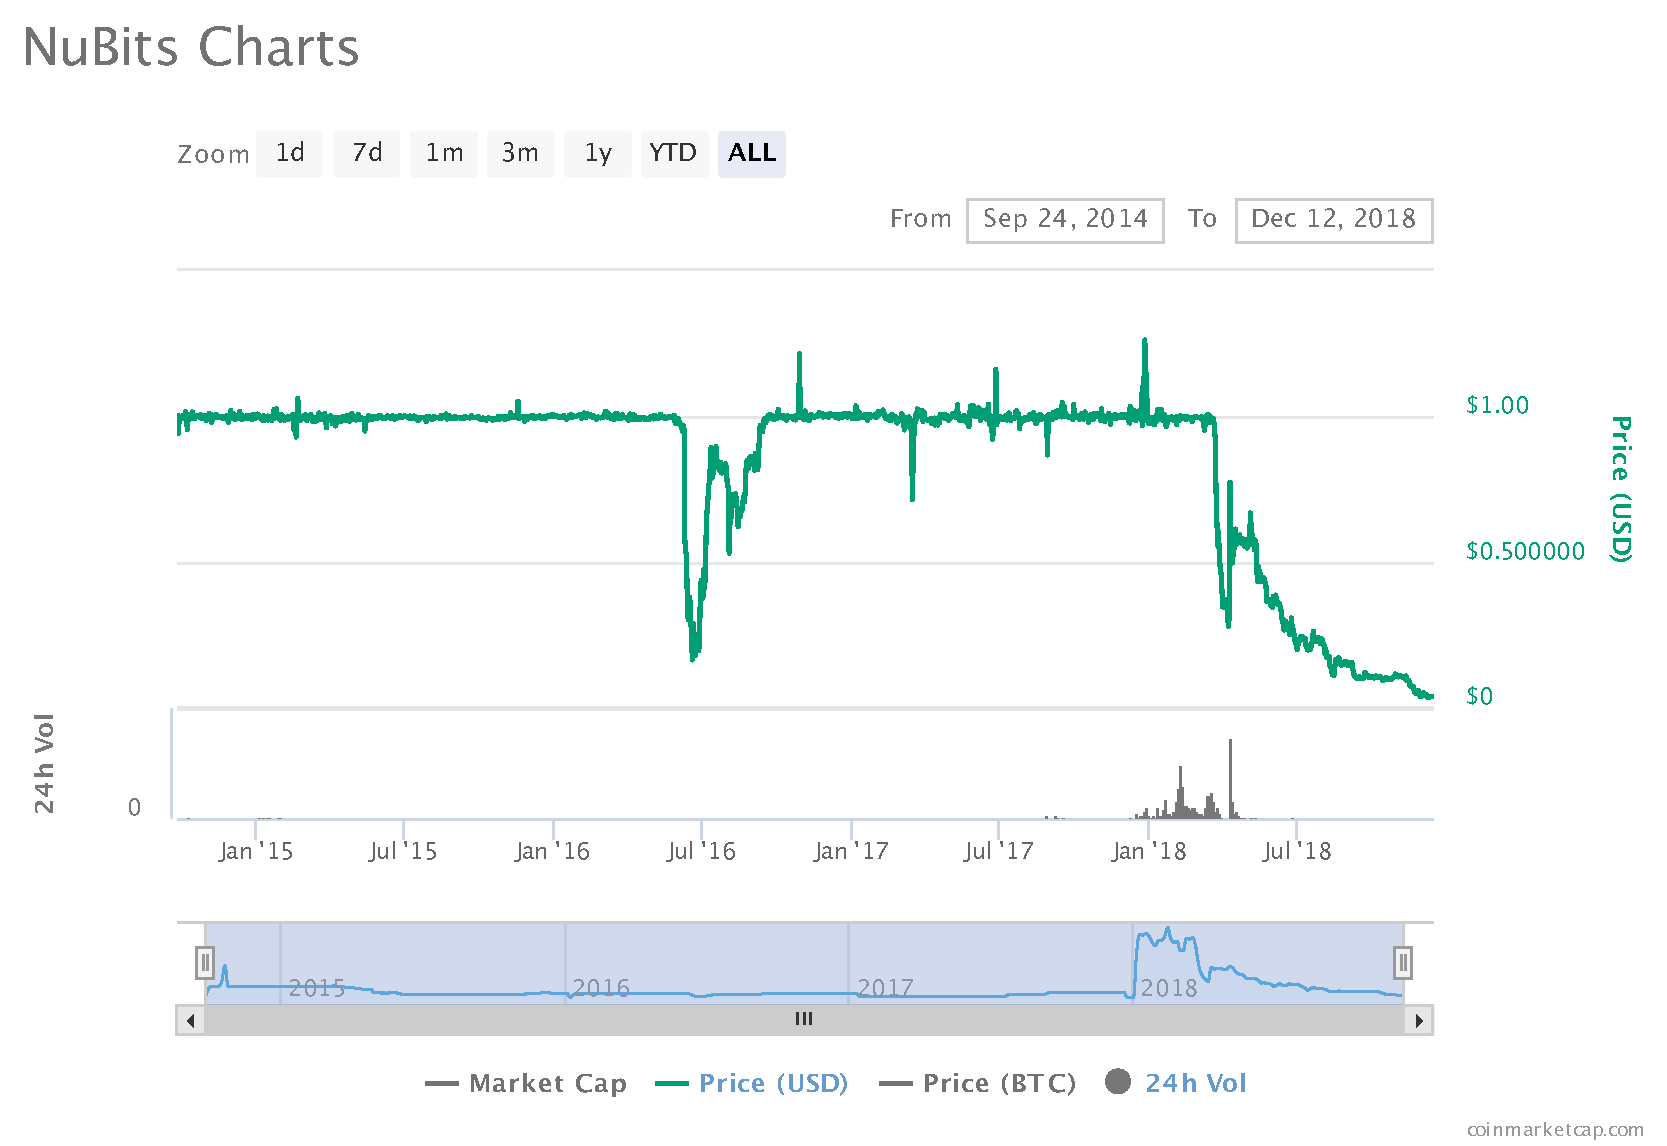
\includegraphics[width=\textwidth]{figures/nubits_chart}
		\caption{NuBits trades at cents on the dollar.}\label{fig:nubits_chart}
	\end{subfigure}
	%
	\begin{subfigure}[b]{0.4\textwidth}
		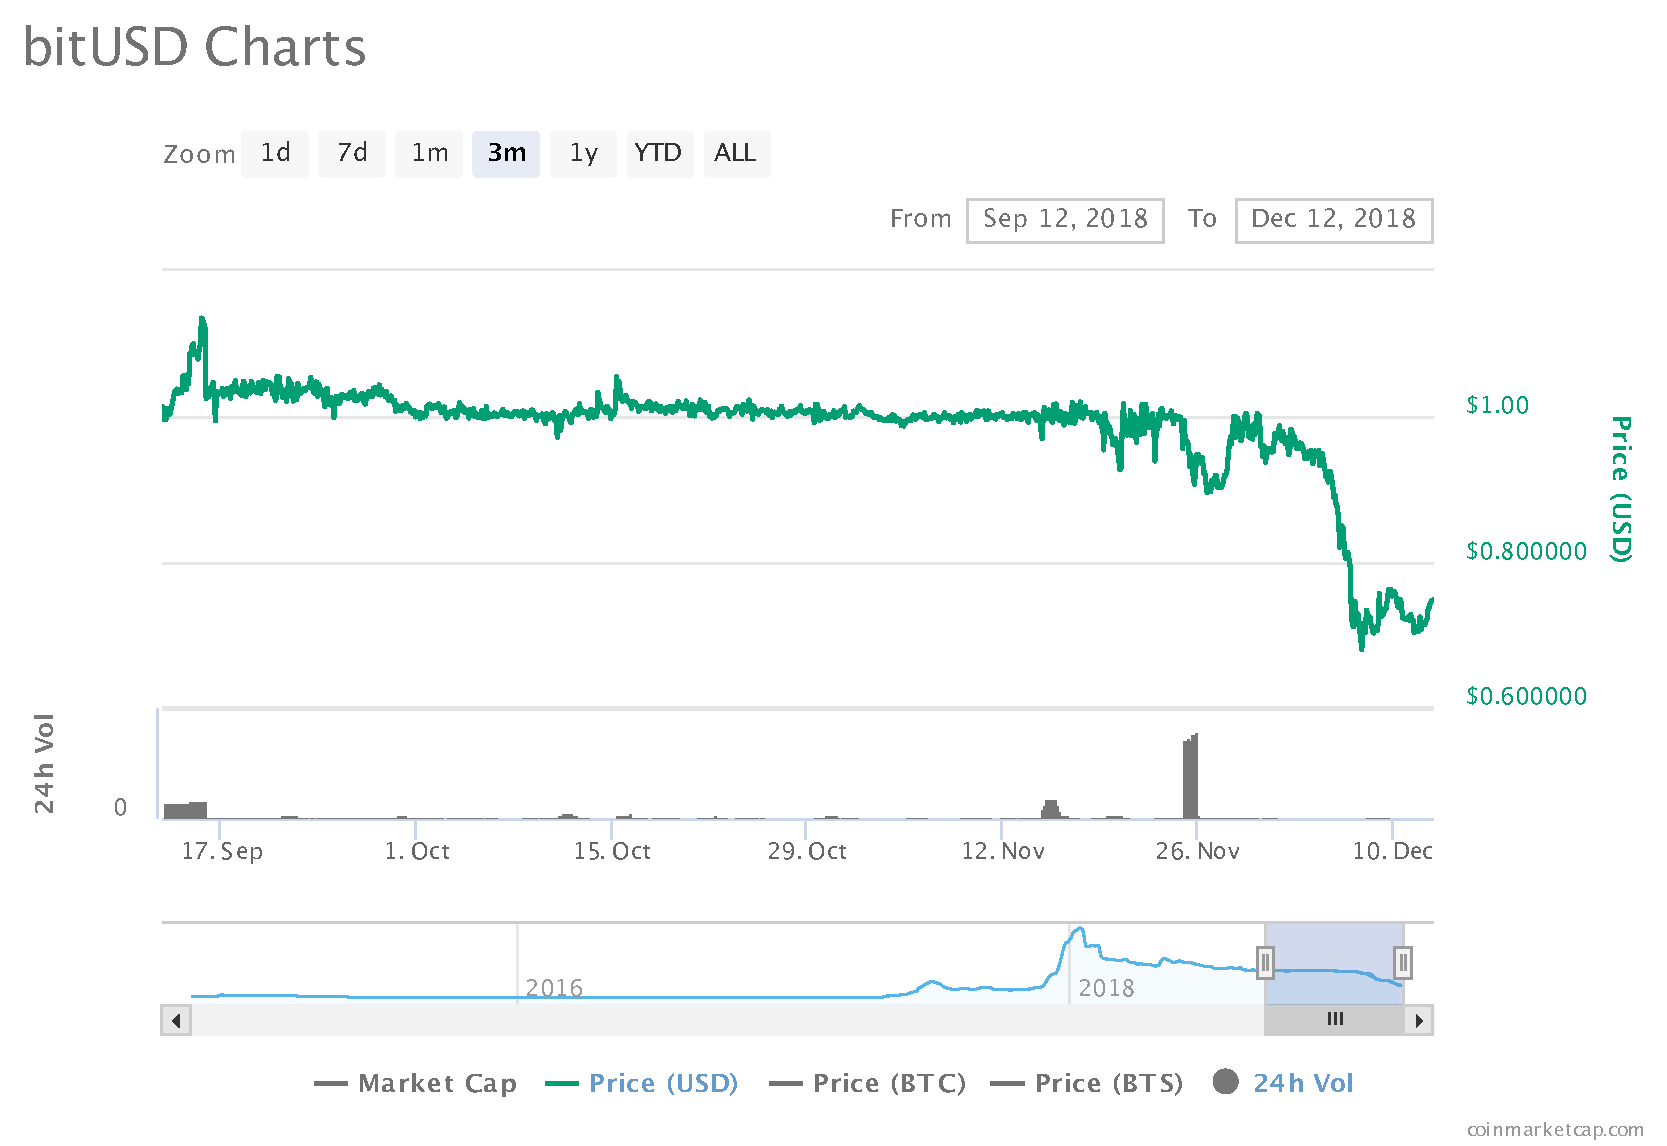
\includegraphics[width=\textwidth]{figures/bitusd_chart}
		\caption{BitUSD has broken its USD peg.}\label{fig:bitusd_chart}
	\end{subfigure}
	\caption{Depeggings in decentralized stablecoins.}
\end{figure}




\subsection{Relation to prior work}

Stablecoins are active cryptocurrencies, for which pre-existing models do not understand how the collateral rule enforces stability and how the interaction of different agents can affect stability.

With the notable exception of \cite{cao2018}, rigorous mathematical work on non-custodial stablecoins is lacking. They applied option pricing theory to valuing tranches in their proposed DStablecoin design using advanced PDE methods. In doing so, they need the simplifying assumption that DStablecoin payouts (e.g., from interest/fee payments and liquidations from leverage resets) are exogenously stable with respect to USD. This may circularly cause stability. In reality, these payouts are made in volatile cryptocurrency (ETH). From these ETH payments, stablecoin holders can
\begin{enumerate}
	\item Hold ETH and so take on ETH exposure,
	\item Use the ETH to re-buy into stablecoin, likely at an inflated price as it endogenously increases demand after a supply contraction,
	\item Convert the ETH to fiat, which requires waiting for block confirmations in an exchange (possibly hours) during times when ETH is particularly volatile and paying costs for fiat conversion (fees, potentially taxes). Notably, this is not available in all jurisdictions.
\end{enumerate}
To maintain a DStablecoin position, stablecoin holders need to re-buy into DStablecoins at each reset at endogenously higher price. Stablecoin holders additionally face the risk that the size of the DStablecoin market collapses such that the position cannot be maintained (and so ends up holding ETH). As no stable asset models exist to understand these endogenous effects, the analysis can't be easily extended using the traditional financial literature.\footnote{A secondary issue with their continuous model is that these systems are inherently discontinuous due to the discrete nature of incorporating blockchain transactions into blocks. Thus resets can occur beyond the set thresholds.} Our focus in this paper is complementary to understand these endogenous stable asset effects.

\cite{lipton2018} studied the evolution of custodial stablecoins. 
A few works on stablecoins have also arisen since the initial release of our paper.
\cite{klagesmundt2019vuln} described governance attack surfaces in non-custodial stablecoins, which is extended with general models in \cite{klagesmundt2020stablecoins}. \cite{evans2019ratings} presented an analysis of credit risk stemming from collateral type in the Maker system. And \cite{terra2, celo} modeled stability in the Terra and Celo stablecoins under different scenarios of Brownian motion without the endogenous market feedback effects we study in this paper.

In the context of central counterparty clearinghouses, the default fund contributions, margin requirements and participation incentives have been studied in, e.g., \cite{capponi2017}, \cite{amini2015}, and \cite{duffie2015}. The critical question in this area is understanding the effects of a liquidation policy of a member's portfolio in the case of a significant event. The counterpart of this in a decentralized setting is understanding the impact of DStablecoin deleveraging on system stability.


Stablecoin holders bear some resemblance to agents in currency peg and international finance models, e.g., \cite{morris1998} and \cite{guimaraes2007}. In these models, the market maker is essentially the government but is modeled with mechanical behavior and is not a player in the game. For instance, in \cite{guimaraes2007}, devaluation is modeled by a simple exogenous threshold rule: the government abandons the peg if the net demand for currency breaches the threshold and is otherwise committed to maintaining the peg. In contrast to currency markets, no agents are committed to maintaining the peg in DStablecoin markets. The best we can hope is that the protocol is well-designed and that the peg is maintained with high probability through the protocol's incentives. The role of government is replaced by decentralized speculators, who issue and withdraw stablecoins in a way to optimize profit. A fully strategic model would be a complicated dynamic game--these tend to be intractable and, indeed, are avoided in the currency peg literature in favor of a sequence of one period games. We enable a more endogenous modeling of speculators' optimization problems under a variety of risk constraints. Our model is a sequence of one-period optimization problems, in which dynamic coupling comes through the risk constraints.

DStablecoin speculators are similar to market makers in market microstructure models (e.g., \cite{ohara1997}). Like classical market microstructure, we do have a multi-period system with multiple agents subject to leverage constraints that take recurring actions according to their objectives. In contrast, in the DStablecoin setting, we do not have a truly stable asset that is efficiently and instantaneously available. Instead, agents make decisions that endogenously affect the price of the `stable' asset and affect the agents' future decisions and incentives to participate in a non-stationary way. In turn, the (in)stability results from the dynamics of these decisions.

Since the initial release of our paper in June 2019, \cite{klagesmundt2020} has described a complementary model of non-custodial stablecoins related to the model in this paper. That paper explores a different model of liquidation structure that affects speculator decision-making and applies martingale methods to analytically characterize stability. In contrast, in this paper we derive stability results about a simpler model that is more amenable to simulations, which we perform, and demonstrate stablecoin attacks that can arise from profitable bets against other agents.






\subsection{This paper}
We develop a dynamic model for non-custodial stablecoins that is complex enough to take into account the feedback effects discussed above and yet remains tractable. Our model can be interpreted as a market microstructure model in this new type of asset market.

Our model involves agents with different risk profiles; some desire to hold stablecoins and others speculate on the market. These agents solve optimization problems consistent with a wide array of documented market behaviors and well-defined financial objectives. As is common in the literature on market microstructure and currency peg games, these agents' objectives are myopic. These objectives are coupled for non-myopic risk using a flexible class of rules that are widely established in financial markets; these allow us to model the effects of a range of cyclic and counter-cyclic behaviors. The exact form of these rules is selected and self-imposed by speculators to match their desired responses and not part of the stablecoin protocol. Thus well-established manipulation of similar rules as applied to traditional financial regulation is not a problem here. Our model goes largely beyond a one-period model. We introduce this model with supporting rationale for design choices in Section~\ref{sec:model}.


Using our model, we make the following contributions:
\begin{itemize}
	\item We derive fundamental results about dynamics and liquidity in our model (Section\ref{sec:dynamics}).
	
	\item We demonstrate that stablecoins face deleveraging feedback effects that may cause illiquidity during crises and exacerbate collateral drawdown (Section~\ref{sec:deleveraging}).
	
	\item We characterize stable dynamics of the system under certain conditions that guarantee no liquidity crash (Section~\ref{sec:stable_v_unstable}) and show instability can occur in simulations outside of this setting (Section~\ref{sec:instability}).
	
	\item We simulate a wide range of market behaviors and find that speculator behavior has a large effect on realized volatilities, but that stablecoin failure times are largely determined by underlying asset movements (Section~\ref{sec:simulations}).
	
	\item We describe new attacks that exploit arbitrage-like opportunities around stablecoin liquidations (Section~\ref{sec:attacks}).
\end{itemize}
We relate these results to historical stablecoin events and apply these insights to suggest design improvements that aim to improve long-term stability. Based on these insights, we also suggest that interactions between multiple speculators and attackers may be the most interesting relationships to explore in more complex models.